
%Talk given virtually to Mac Hyman and friends, November 15, 2021
\documentclass[10pt,compress,xcolor={usenames,dvipsnames},aspectratio=169]{beamer}
%\documentclass[xcolor={usenames,dvipsnames},aspectratio=169]{beamer} %slides and 
%notes
\usepackage{amsmath,
	amssymb,
	datetime,
	mathtools,
	bbm,
	%mathabx,
	array,
	booktabs,
	xspace,
	multirow,
	calc,
	colortbl,
	siunitx,
 	graphicx}
\usepackage[usenames]{xcolor}
\usepackage[giveninits=false,backend=biber,style=nature, maxcitenames =10, mincitenames=9]{biblatex}
\addbibresource{FJHown23.bib}
\addbibresource{FJH23.bib}
\usepackage{newpxtext}
\usepackage[euler-digits,euler-hat-accent]{eulervm}
\usepackage{media9}
\usepackage[autolinebreaks]{mcode}
\usepackage[tikz]{mdframed}


\usetheme{FJHSlimNoFoot169}
\setlength{\parskip}{2ex}
\setlength{\arraycolsep}{0.5ex}


\DeclareMathOperator{\SOL}{SOL}
\DeclareMathOperator{\APP}{APP}
\DeclareMathOperator{\ERR}{ERR}
\DeclareMathOperator{\AVG}{AVG}
\DeclareMathOperator{\INT}{INT}
\DeclareMathOperator{\LIN}{LINEAR}
\DeclareMathOperator{\BAD}{BAD}
%\DeclareMathOperator{\opt}{opt}
\newcommand{\dataN}{\bigl(\hf(\vk_i)\bigr)_{i=1}^n}
\newcommand{\dataNj}{\bigl(\hf(\vk_i)\bigr)_{i=1}^{n_j}}
\newcommand{\dataNjd}{\bigl(\hf(\vk_i)\bigr)_{i=1}^{n_{j^\dagger}}}
\newcommand{\ERRN}{\ERR\bigl(\dataN,n\bigr)}
\newcommand{\otod}{\ensuremath{1\mkern-4mu : \mkern-2mu d}}


%\DeclareMathOperator{\app}{app}

\providecommand{\HickernellFJ}{H.\xspace}


\renewcommand{\OffTitleLength}{-7ex}
\setlength{\FJHThankYouMessageOffset}{-8ex}
\title{Reproducing Kernels, Function Spaces, Measures, Distributions}
\author[]{Fred J. Hickernell and Aleksei Sorokin}
\institute{Department of Applied Mathematics \qquad
	Center for Interdisciplinary Scientific Computation \\
	Office of Research \\  
	Illinois Institute of Technology \qquad
	\href{mailto:hickernell@iit.edu}{\url{hickernell@iit.edu}} \qquad
	\href{http://mypages.iit.edu/~hickernell}{\url{mypages.iit.edu/~hickernell}}}

\thanksnote{Thanks to those helping us clarify these ideas \\
Slides available at \href{https://speakerdeck.com/fjhickernell/reproducing-kernel-tutorial}{\nolinkurl{speakerdeck.com/fjhickernell/reproducing-kernel-tutorial}} \\
Please interrupt and ask questions}
	
%\event{Happy Fred}
\date[]{ revised \today}

\input FJHDef.tex



\begin{document}
	\everymath{\displaystyle}

\frame{\titlepage}

%%%%%%%%%%%%%%%%%%%%%%%%%%%%%%%%%%%%%%%%%%
%%%%%%%%%%%%%%%%%%%%%%%%%%%%%%%%%%%%%%%%%%
\section{Background}
%%%%%%%%%%%%%%%%%%%%%%%%%%%%%%%%%%%%%%%%%%
%%%%%%%%%%%%%%%%%%%%%%%%%%%%%%%%%%%%%%%%%%

\begin{frame}{What to Do with Reproducing Kernels}

\vspace{-5ex}
	\begin{itemize}
		\item Uniquely identified Hilbert spaces of functions, $\cf$, for which function evaluation at any point $\vx$ is a bounded functional
		\item Use the Reisz Representation Theorem to derive error bounds for algorithms for linear problems, such as integration, function approximation, and solving linear differential equations%
		\item Derive optimal algorithms by optimizing the weights and the data sites%
		\item Determine how fast the error bounds decay to zero, and even whether convergence depends significantly on the number of variables
		\item Derive a parallel analysis using Gaussian processes where the reproducing kernel is interpreted as a covariance kernel
	\end{itemize}	

\end{frame}

\begin{frame}{Reproducing Kernels for Functions on General Domains  \cite{Aro50}}
	
	\vspace{-4ex}
	Suppose that  $(\cf,\ip{\cdot}{\cdot})$  is a Hilbert space of functions on $\Omega$ for which \alert{function evaluation is bounded}.  Then there exists a \alert{unique reproducing kernel}  $K: \Omega \times \Omega \to \reals$ for which 
	\vspace{-1ex}
	\begin{gather*}
		\underbrace{K(\vt,\vx) = K(\vx,\vt)}_{\alert{\text{symmetry}}},  \quad \underbrace{K(\cdot,\vx) \in \cf}_{\alert{\text{belonging}}}, \quad  \underbrace{f(\vx) = \ip{K(\cdot,\vx)}{f}}_{\alert{\text{reproduction}}}  \qquad \forall \vt, \vx \in \Omega, \; f \in \cf \\
		K(\mX,\mX) = \bigl(K(\vx_i,\vx_j)\bigr)_{i,j = 1}^n \text{ is \alert{positive definite} for any $n \times d$ $\mX$ with distinct rows lying in $\Omega$}
	\end{gather*}
	
	$\cf$ is the completion of the pre-Hilbert space, $\cf_0 := \{c_1 K(\cdot,\vx_1) + \cdots + c_nK(\cdot, \vx_n) : n \in \naturals, \vc \in \reals^n\}$; any $K$ satisfying the above implies $\cf$
	
	Reproducing kernels are \alert{unique}. If $\eta_\vx \in \cf$ is the representer for function evaluation at  $\vx \in \Omega$, then 
	\[
	K(\vt,\vx) := \ip{\eta_\vt}{\eta_\vx} = \eta_\vt(\vx) = \eta_\vx(\vt)
	\]
	
\end{frame}


%%%%%%%%%%%%%%%%%%%%%%%%%%%%%%%%%%%%%%%%%%
%%%%%%%%%%%%%%%%%%%%%%%%%%%%%%%%%%%%%%%%%%
\section{Kernel Ex}
%%%%%%%%%%%%%%%%%%%%%%%%%%%%%%%%%%%%%%%%%%
%%%%%%%%%%%%%%%%%%%%%%%%%%%%%%%%%%%%%%%%%%

\begin{frame}[label = RKRd]{Reproducing Kernels for Functions on $\{1, \ldots, d\}$, aka Vectors}
	
	\vspace{-3ex}
	Let $\cf:=$ all functions on $\Omega := \{1, \ldots, d\} \text{ ``$=$'' } \reals^d$
	
	Pick a symmetric, positive definite (positive eigenvalues) matrix $\mW \in \reals^{d \times d}$ to define an inner product \vspace{-0.3ex}
	\[
	\ip{f}{h} : = \vf^T \mW \vh, \quad \forall f, h \in \cf, \qquad \text{where } \vf = \bigl(f(t) \bigr)_{t=1}^d
	\]
	\alert{Reproducing kernel}, $K$, is defined by 
			$\bigl ( K(t,x) \bigr)_{t,x=1}^d = \mK := \mW^{-1}$, and has the properties
		\vspace{-0.5ex}
		\begin{gather*}
			\alert{\text{Symmetry }} K(t,x) = K(x,t) \text{ because $\mW$ is symmetric and thus so is $\mK$} \\
			\alert{\text{Positive Definiteness }} \bigl(  K(x_i,x_j)\bigr)_{i,j = 1}^n \text{ is positive definite for any distinct } x_1, \ldots, x_n \in \{1, \ldots, d\}\\
			\alert{\text{Belonging }} K(\cdot,x) = \text{$x^{\text{th}}$ column of $\mK$} =: \vK_x \in \cf\\
			\alert{\text{Reproduction }} \ip{K(\cdot,x)}{f} = \vK_x^T \mW \vf = \ve_x \vf = f(x) \quad \text{since } \mK := \mW^{-1};  \qquad 
				\ve_x := (0, \ldots, 0, \underbrace{1}_{x^{\text{th}} \text{ position}}, 0, \ldots )^T
		\end{gather*}
	
	
\end{frame}
\begin{frame}{Squared Exponential Kernel on $\reals$}
	
	\begin{tabular}{m{0.5\textwidth}m{0.5\textwidth}}
		The squared exponential (aka Gaussian) kernel for univariate functions takes the form 
		\[
		K(t,x) = A \exp\bigl(-\gamma^2\abs{t-x}^2 \bigr) , \qquad t, x \in \reals
		\]
		corresponds to the Hilbert space of functions with norm \cite[(6.18)]{RasWil06a}
		\begin{equation*}
			\norm{f}^2 = A\sqrt{\pi} \sum_{m=0}^\infty\frac{\int_{\reals} \abs{f^{(m)}(x)}^2 \, \dif x}{m! 4^m \gamma^{2m+1}}
		\end{equation*}
		which means that functions  have all deriviatives square integrable.
		&
		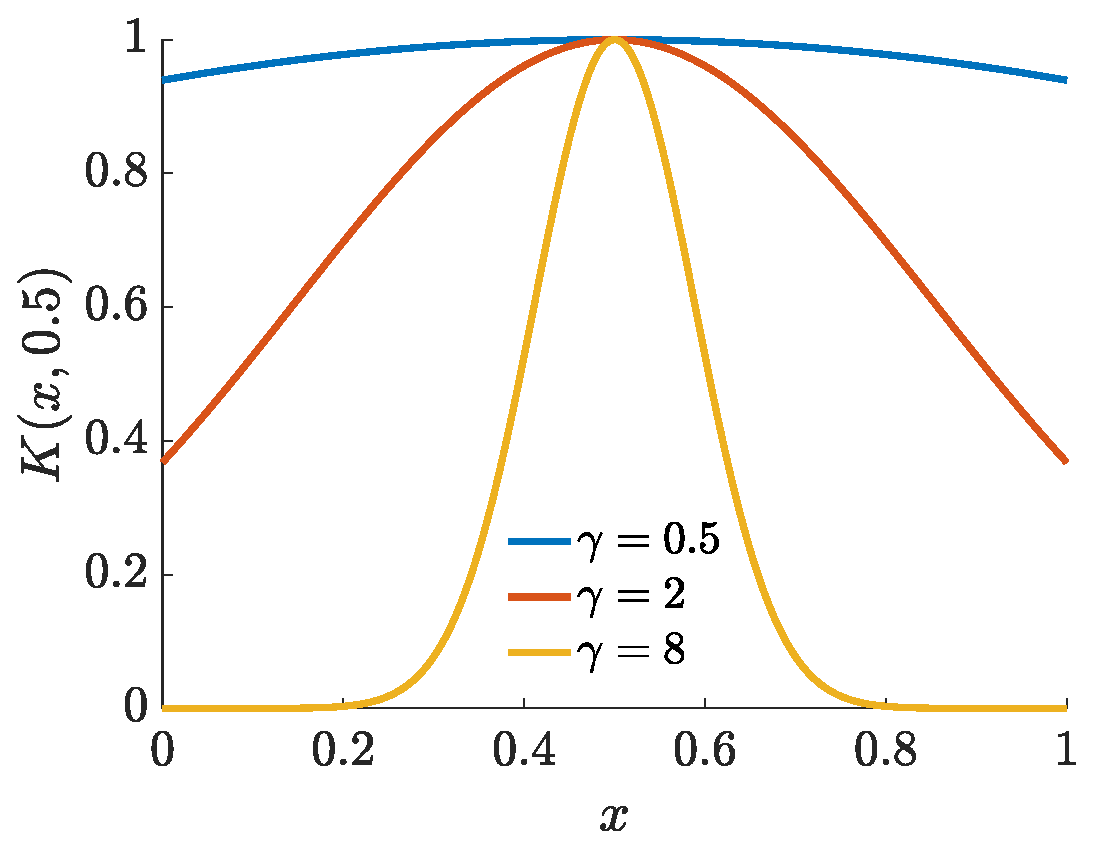
\includegraphics[width=0.45\textwidth]{RK-sqexpker.eps}
	\end{tabular}
\end{frame}

\begin{frame}{Squared Exponential Kernel on $\reals^d$}
	\begin{tabular}{m{0.6\textwidth}m{0.4\textwidth}}
		The squared exponential kernel for $d$-variate functions takes the form 
		\begin{multline*}
			K(t,x) = A \exp\bigl(-\gamma_1^2\abs{t_1-x_1}^2 - \cdots - \gamma_d^2\abs{t_d-x_d}^2 \bigr) , \\
			t, x \in \reals
		\end{multline*}
		corresponds to the Hilbert space of functions with norm
		\begin{gather*}
			\norm[2]{D^{\vm} f}^2 := \int_{\reals^d} \abs{\frac{\partial^{\norm[1]{\vm}}f(\vx)}{\partial x_1^{m_1} \cdots \partial x_d^{m_d}}}^2 \, \dif \vx \\
			\norm{f}^2 =  A\sqrt{\pi}  \sum_{\vm \in \natzero^d} \frac{\norm[2]{D^{\vm} f}^2}{\norm[1]{\vm}! \, 4^{\norm[1]{\vm}} \prod_{k=1}^d \gamma_j^{2m_j}}
		\end{gather*}
		which means that functions have all deriviatives square integrable.  This kernel is \alert{isotropic}.
		&
		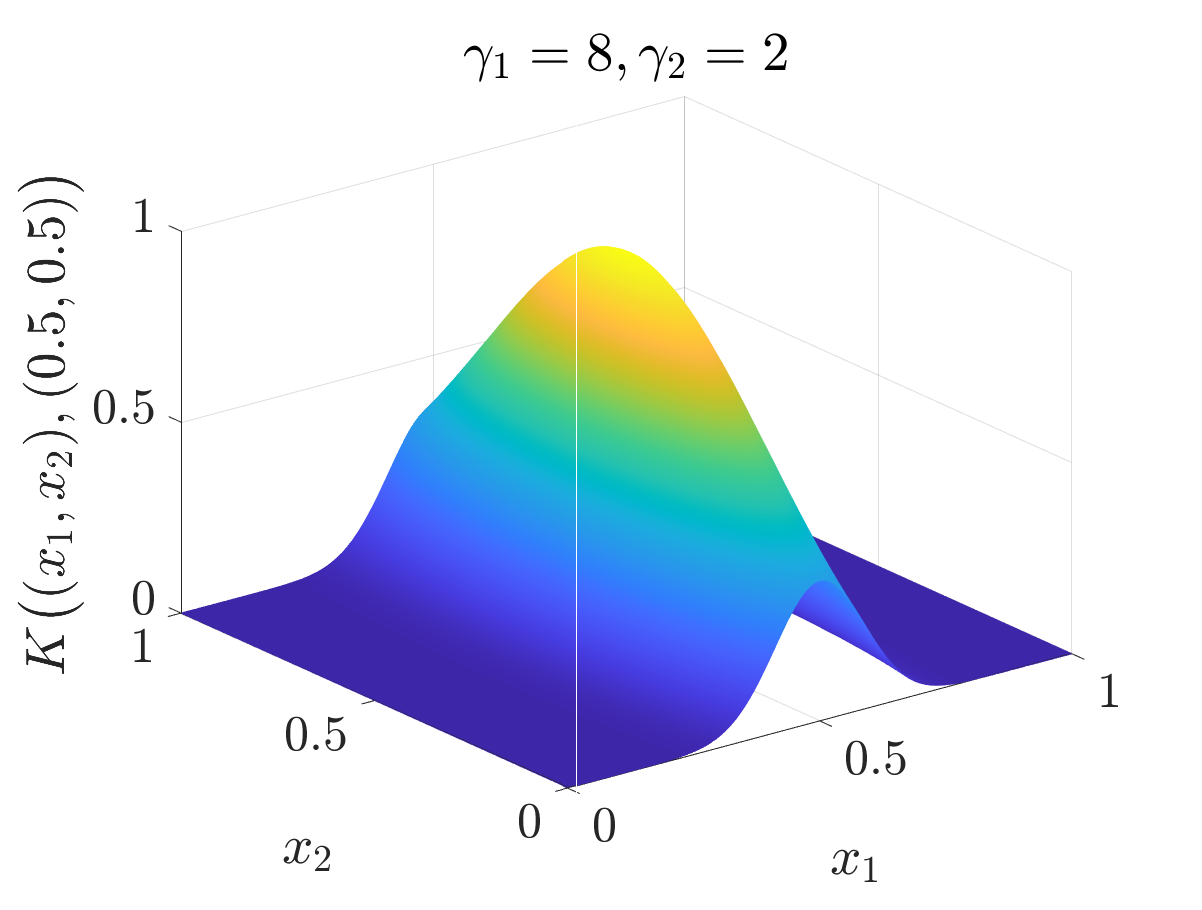
\includegraphics[width=0.38\textwidth]{RK2-sqexpker.eps}
	\end{tabular}
	
\end{frame}

\begin{frame}{Mat\'ern Kernels}
	
	\vspace{-5ex}
	\begin{tabular}{b{0.5\textwidth}p{0.5\textwidth}}
		A popular family of kernels with a range of smoothness depending on $r$ with an associate norm that is not simple to write down:
		& 	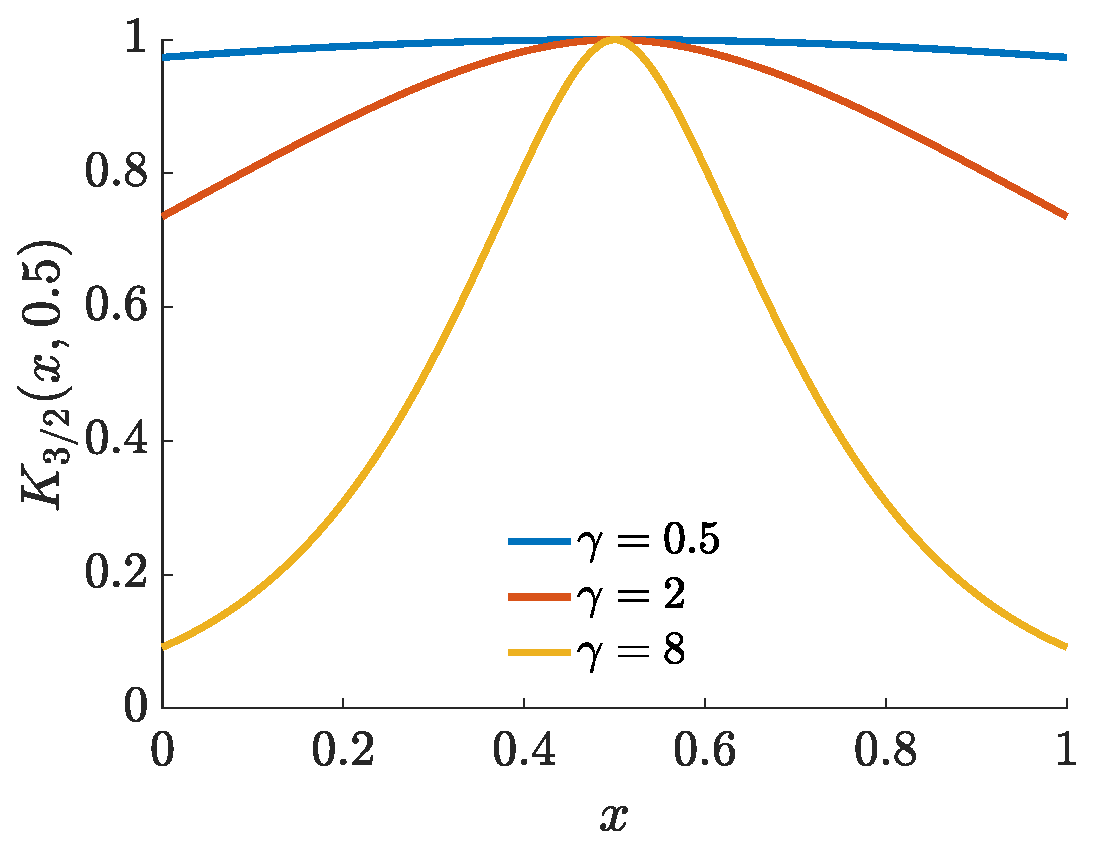
\includegraphics[width=0.45\textwidth]{RK-maternkerthreehalfs.eps}
	\end{tabular}
	\begin{align*}
		K_r(\vt,\vx) &= A \norm[2]{\vt - \vx}^r \text{Mod Bessel Sec}_r (\gamma \norm[2]{\vt - \vx}) \\
		K_{1/2}(\vt,\vx) & = A_{1/2} \exp(-\gamma\norm[2]{\vt - \vx} )  \quad \alert{\text{not very smooth}} \\
		K_{3/2}(\vt,\vx) & = A_{3/2} (1 + \gamma\norm[2]{\vt - \vx} ) \exp(-\gamma\norm[2]{\vt - \vx} )  \quad \alert{\text{somewhat  smoother}}
	\end{align*}
	
	
\end{frame}

\begin{frame}{The Centered Discrepancy Kernel \cite{Hic97a}}
	\vspace{-2ex}
	\begin{tabular}{m{0.6\textwidth}m{0.4\textwidth}}
		A reproducing kernel used to analyze cubatures gives the weighted centered discrepancy takes the form
		
		\vspace{-4ex}
		\begin{multline*}
			K(\vt,\vx) : = \prod_{k=1}^d \Bigl[ 1 + \frac {\gamma_j}2 \bigl\{ \abs{t_k - 1/2} + \abs{x_k -1/2} - \abs{t_k-x_k} \bigr\} \Bigr]. \\
			\vt, \vx \in [0,1]^d
		\end{multline*}
		
		\vspace{-2ex}
		which corresponds to the Hilbert space for functions defined on $[0,1]^d$ with the following norm:
		
		\vspace{-4ex}
		\begin{gather*}
			\norm[2]{D^{\vm} f}^2 := \int_{\reals^d} \abs{\frac{\partial^{\norm[1]{\vm}}f(\vx)}{\partial x_1^{m_1} \cdots \partial x_d^{m_d}}}^2 \bigg \rvert_{x_j = 1/2 \text{ for } m_j = 0} \, \prod_{j \text{ s.t. } m_j > 0} \dif x_j  \\
			\norm{f}^2 : = A \sum_{\norm[\infty]{\vm} \le 1} \frac{\norm[2]{D^{\vm} f}^2}{\gamma_j}
		\end{gather*}
		Mixed partial derivatives of up to order one in each coordinate must be square integrable.
		&
		%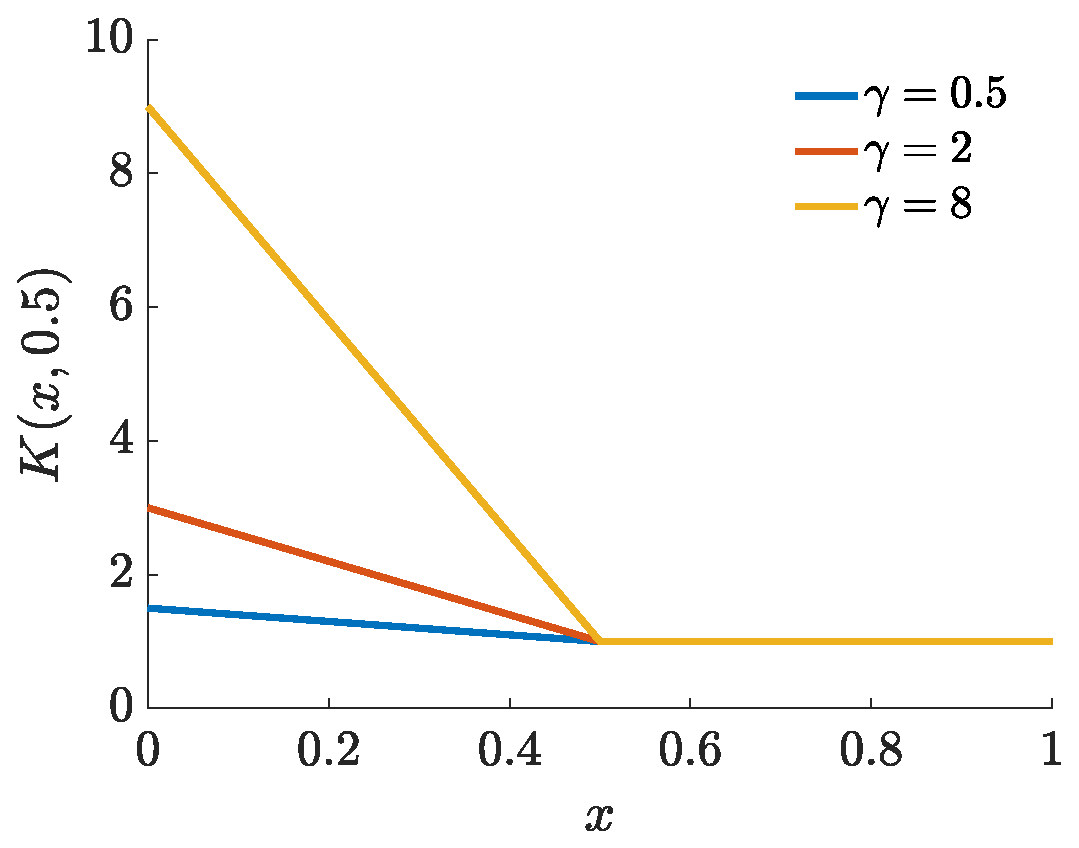
\includegraphics[width=0.38\textwidth]{RK-ctrdiscker.eps}
		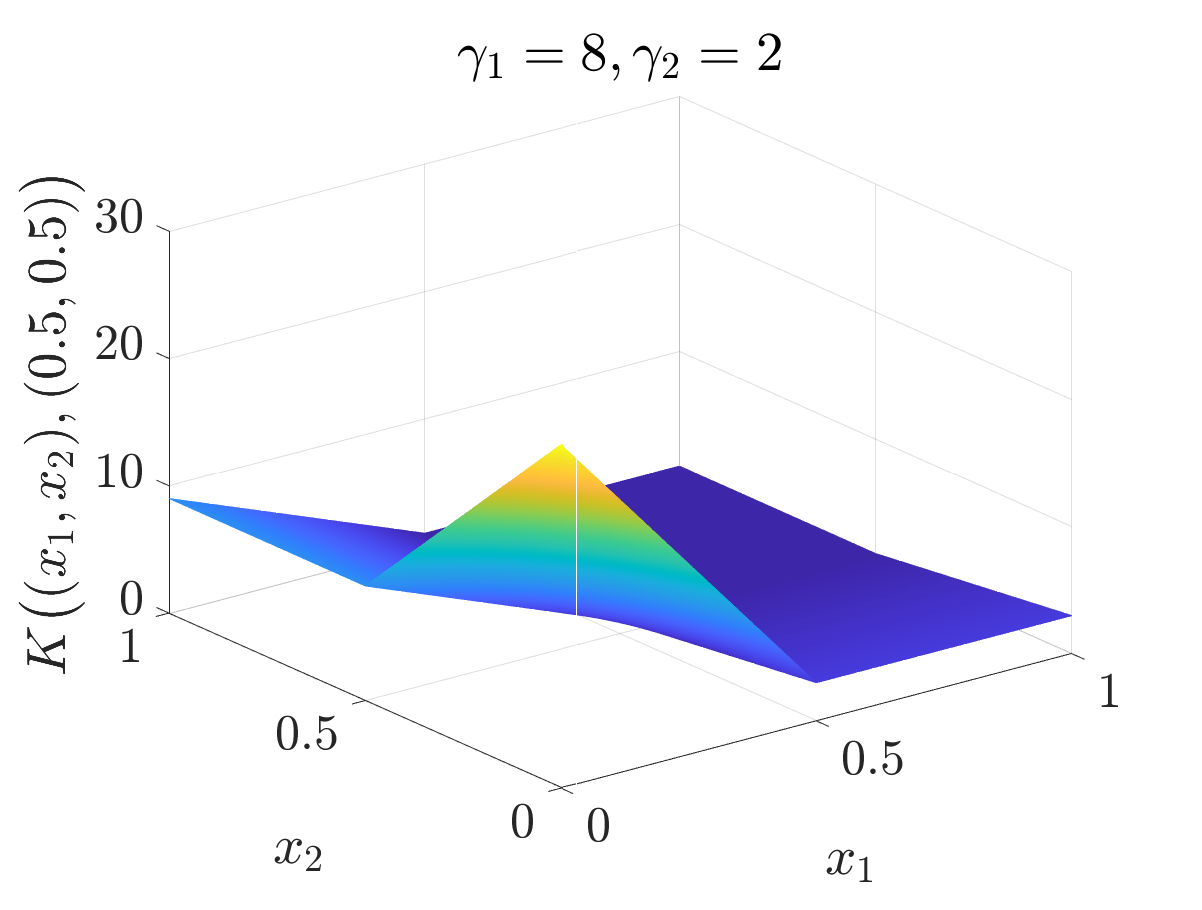
\includegraphics[width=0.38\textwidth]{RK2-ctrdiscker.eps}
	\end{tabular}
\end{frame}


\begin{frame}{The Delta Kernel}
	\vspace{-2ex}
	\begin{tabular}{m{0.5\textwidth}m{0.5\textwidth}}
		A reproducing kernel with an uncountable basis is 
		
		\vspace{-4ex}
		\begin{equation*}
			K(\vt,\vx) : = \begin{cases} 1 + \gamma, & \vt = \vx, \\ 1, & \text{otherwise}, \end{cases}
			\qquad \vt, \vx \in [0,1]^d
		\end{equation*}
		
		\vspace{-2ex}
		which corresponds to the Hilbert space for functions that are a constant everywhere except possibly at a countable number of points.
		
		\vspace{-4ex}
		\begin{gather*}
			I(f) = \int_{[0,1]^d} f(\vx) \, \dif \vx \\
			\norm{f}^2 : = \abs{I(f)}^2 + \sum_{\vx \in [0,1]^d} \frac{\abs{f(\vx) - I(f)}^2}{\gamma}
		\end{gather*}
		This Hilbert space has an \alert{uncountable basis}.
		&
		%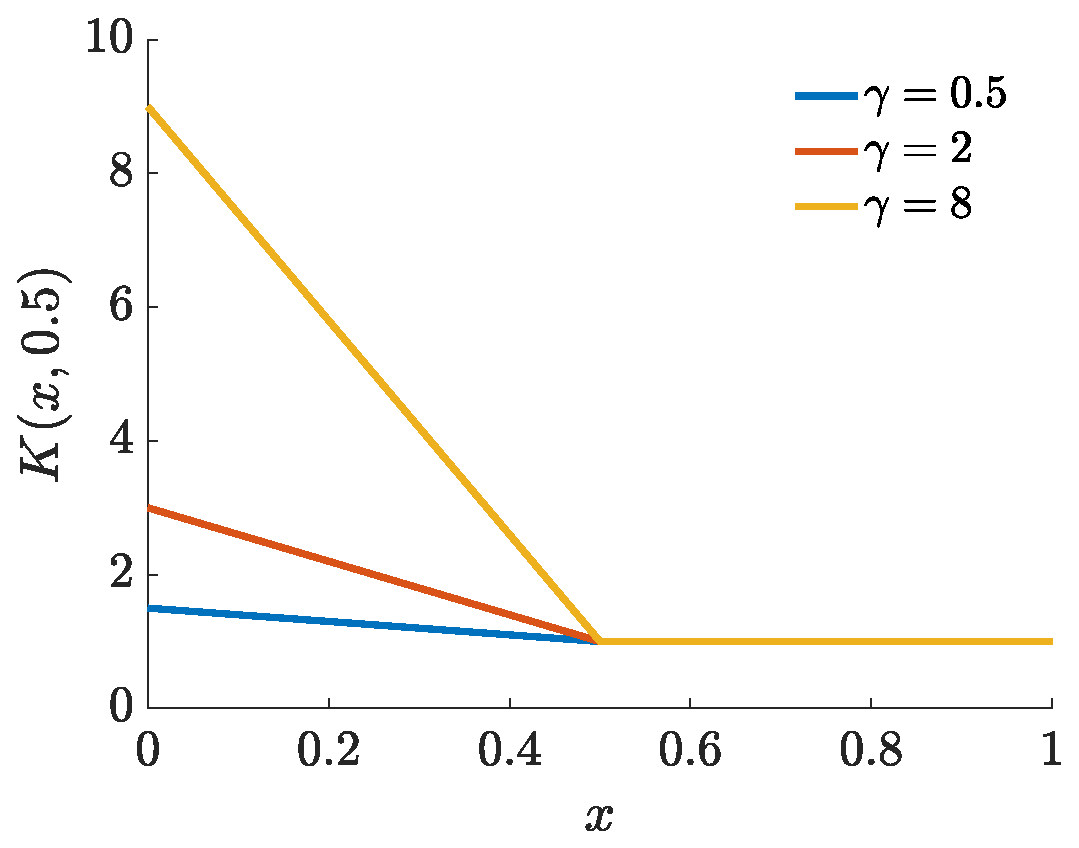
\includegraphics[width=0.38\textwidth]{RK-ctrdiscker.eps}
		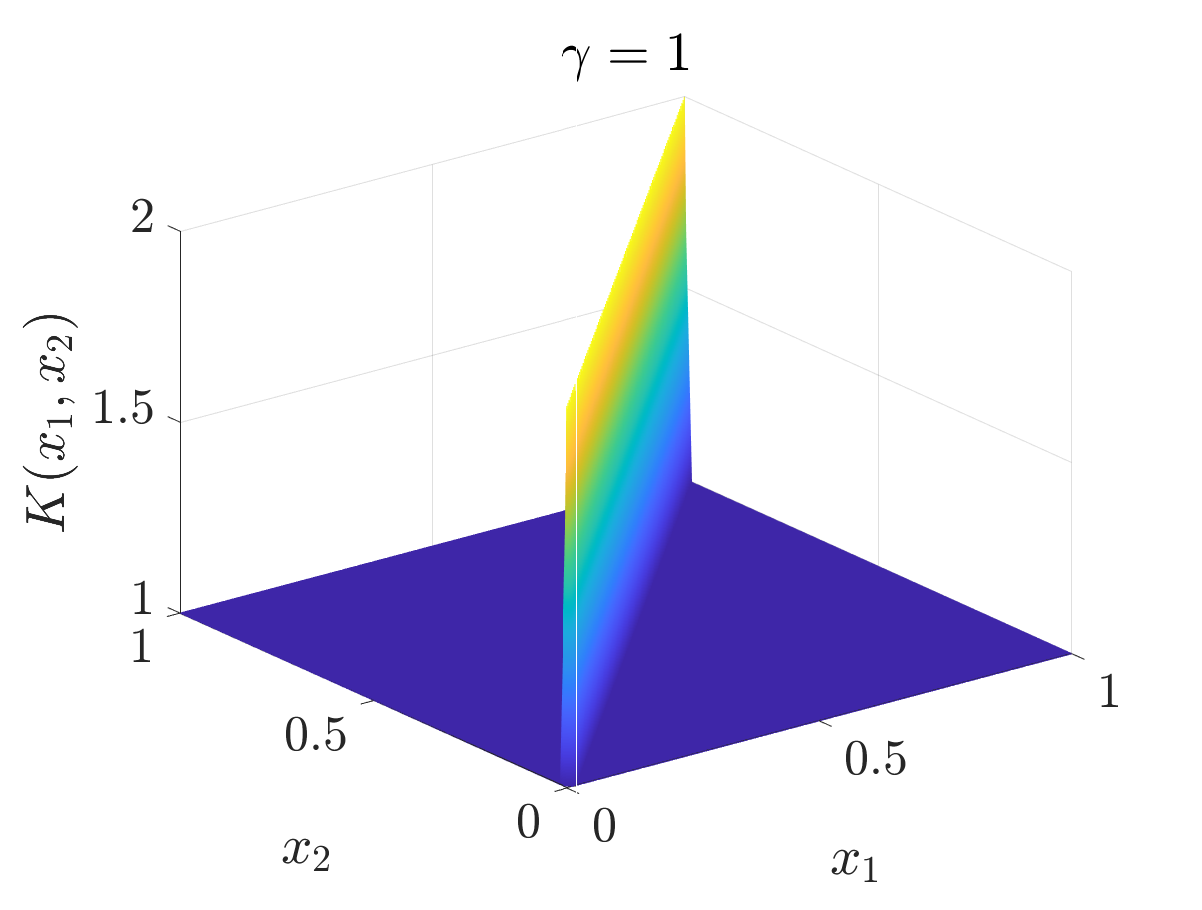
\includegraphics[width=0.38\textwidth]{RK-deltaker.eps}
	\end{tabular}
\end{frame}


%%%%%%%%%%%%%%%%%%%%%%%%%%%%%%%%%%%%%%%%%%
%%%%%%%%%%%%%%%%%%%%%%%%%%%%%%%%%%%%%%%%%%
\section{Riesz Rep Thm}
%%%%%%%%%%%%%%%%%%%%%%%%%%%%%%%%%%%%%%%%%%
%%%%%%%%%%%%%%%%%%%%%%%%%%%%%%%%%%%%%%%%%%

\begin{frame}{Reproducing Kernels Identify Representers}

\vspace{-4ex}
	Suppose that  $(\cf,\ip{\cdot}{\cdot})$  is a Hilbert space of functions on $\Omega$ with \alert{unique reproducing kernel}  $K: \Omega \times \Omega \to \reals$ 
	
Riesz Representation Theorem says that for any bounded $\LIN : \cf \to \reals$ there exists a \alert{representer} $g \in \cf$ such that $\LIN(f)  =  \ip{g}{f} $ for all $f \in \cf$.  \alert{What is $g$?}
\begin{gather*}
	g(\vx) \underbrace{=}_{\text{reproduction}} \ip{K(\cdot,\vx)}{g} \underbrace{=}_{\text{symmetry}}  \ip{g}{K(\cdot,\vx)} \underbrace{=}_{\text{representer}} \LIN\bigl(K(\cdot,\vx)\bigr) \qquad \forall \vx \in \Omega\\
		\norm{g}^2 = \ip{g}{g} \underbrace{=}_{\text{representer}} \LIN(g) = \LIN^{\cdot\cdot} \bigl( \LIN^\cdot\bigl(K(\cdot,\cdot \cdot)\bigr)   \bigr)
\end{gather*}
\vspace{-3ex}
\alert{Do not} need the definition of $\ip{\cdot}{\cdot}$ to compute $g$ and $\norm{g}$

\end{frame}


\begin{frame}{Ex.\ Representer for Functionals on Matrices}

If $\ip{f}{h}$

\end{frame}



\end{document}


%%%%%%%%%%%%%%%%%%%%%%%%%%%%%%%%%%%%%%%%%%
%%%%%%%%%%%%%%%%%%%%%%%%%%%%%%%%%%%%%%%%%%
\section{Rep Ker \& Riesz Rep Thm}
%%%%%%%%%%%%%%%%%%%%%%%%%%%%%%%%%%%%%%%%%%
%%%%%%%%%%%%%%%%%%%%%%%%%%%%%%%%%%%%%%%%%%

\begin{frame}[label = RKRd]{Reproducing Kernels for Functions on $\{1, \ldots, d\}$, aka Vectors}

\vspace{-3ex}
Let $\cf$ \uncover<1-3>{$:=$ all functions on $\{1, \ldots, d\} \text{ ``$=$'' } \reals^d$}\uncover<4>{ be a vector space of functions}\\
\uncover<1-3>{Pick a symmetric, positive definite (positive eigenvalues) matrix $\mW \in \reals^{d \times d}$ to} define an inner product \vspace{-0.3ex}
\[
\only<1-3>{\ip{f}{h} : = \vf^T \mW \vh, \quad \forall f, h \in \cf, \qquad \text{where } \vf = \bigl(f(t) \bigr)_{t=1}^d} \only<4>{\alert{\mW \text{ is gone}}} \vspace{-0.7ex}
\]
\uncover<2-4>{\alert{Reproducing kernel}, $K$, \uncover<1-3>{is defined by 
$\bigl ( K(t,x) \bigr)_{t,x=1}^d = \mK := \mW^{-1}$, and }has the properties
\vspace{-0.5ex}
\begin{gather*}
    \alert{\text{Symmetry }} K(t,x) = K(x,t) \uncover<1-3>{\text{ because $\mW$ is symmetric and thus so is $\mK$}} \\
    \alert{\text{Positive Definiteness }} \bigl(  K(x_i,x_j)\bigr)_{i,j = 1}^n \text{ is positive definite for any distinct } x_1, \ldots, x_n \in \{1, \ldots, d\}\\
     \alert{\text{Belonging }} K(\cdot,x)\uncover<1-3>{ = \text{$x^{\text{th}}$ column of $\mK$} =: \vK_x} \in \cf\\
    \alert{\text{Reproduction }} \ip{K(\cdot,x)}{f} \uncover<1-3>{= \vK_x^T \mW \vf = \ve_x \vf} = f(x) \uncover<1-3>{\quad \text{since } \mK := \mW^{-1};  \qquad 
 \ve_x := (0, \ldots, 0, \underbrace{1}_{x^{\text{th}} \text{ position}}, 0, \ldots )^T}
\end{gather*}
\uncover<3->{\alert{Riesz Representation Theorem} says that \uncover<1-3>{for any linear function, $\LIN$, there is a \alert{representer} $g$ such that} $\LIN(f) = \ip{g}{f}\uncover<1-3>{ = \vg^T \mW \vf}$\uncover<1-3>{.  Note}
\[
\begin{pmatrix} g(1) \\ \vdots \\ g(d)\end{pmatrix} 
\uncover<1-3>{= \vg = \mK \mW \vg 
= \begin{pmatrix} \mK_1^T \mW \vg \\ \vdots \\ \mK_d^T \mW \vg\end{pmatrix}
= \begin{pmatrix} \ip{K(\cdot,1)}{g} \\ \vdots \\ \ip{K(\cdot,d)}{g} \end{pmatrix}}
= \begin{pmatrix} \LIN(K(\cdot,1)) \\ \vdots \\  \LIN(K(\cdot,d)) \end{pmatrix}
\]
}
}


\end{frame}






%%%%%%%%%%%%%%%%%%%%%%%%%%%%%%%%%%%%%%%%%%
%%%%%%%%%%%%%%%%%%%%%%%%%%%%%%%%%%%%%%%%%%
\section{Assoc Measures}
%%%%%%%%%%%%%%%%%%%%%%%%%%%%%%%%%%%%%%%%%%
%%%%%%%%%%%%%%%%%%%%%%%%%%%%%%%%%%%%%%%%%%




\begin{frame}{Hilbert Spaces of Signed Measures}
	
	\vspace{-4ex}
	Let $\cm$ be the Hilbert spaced of  measures on $\Omega$ that is the completion of $\{c_1 \delta_{\vx_1} + \cdots + c_n \delta_{\vx_n} :  n \in \naturals, \vc \in \reals^n \}$ under the norm induced by
	\begin{equation*}
		\ip[\cm]{\mu}{\nu} := \int_{\Omega \times \Omega} K(\vt,\vx) \, (\mu \times \nu) (\dif \vt \times \dif \vx)
	\end{equation*}
	and $\delta_{\vx}$ is the Dirac measure, i.e., $\int_{\Omega} f(\vt) \, \delta_\vx(\dif \vt) = f(\vx)$.  There exists a one-to-one and onto, isometric  (I think) mapping $T : \cm \to \cf$ defined as 
		\begin{equation*}
			T(\mu)(\vx) := \int_\Omega K(\vt, \vx) \, \mu(\dif t) \qquad \forall x \in \Omega, \mu \in \cm
		\end{equation*}
Good question:  is there a measure $\omega $ on $\Omega \times \Omega$ such that 
		\begin{equation*}
      \int_{\Omega \times \Omega} K(\vt, \vs)K(\vu,\vx) \, \omega(\dif \vs \times \dif \vu)  = K(\vt,\vx) \qquad \forall \vt, \vx \in \Omega?
\end{equation*}
This would be like the $\mW$ for functions on $\{1, \ldots, d\}$

\end{frame}

\begin{frame}{Hilbert Spaces with Countable Bases}
	
\vspace{-4ex}
Hilbert spaces of functions on $\Omega$ with countable bases can be written in terms of an $L^2(\Omega)$ basis

\vspace{-4ex}
\[
f(\vx) = \sum_{\vk} \hf(\vk) \varphi_\vk(\vx), \qquad \int_\Omega \varphi_\vk(\vx) \varphi_\vl(\vx)  \, \dif \vx = \delta_{\vk,\vl}
\]

\vspace{-2ex}
and the reproducing kernel is
\vspace{-2ex}
\begin{gather*}
K(\vt,\vx) =  \sum_{\vk} \lambda_\vk \varphi_\vk(\vt) \varphi_\vk(\vx),  \qquad
\text{note that }  \int_\Omega K(\vx,\vx) \, \dif \vx = \sum_{\vk} \lambda_\vk  < \infty, \quad \text{so } \lambda_{\vk} \to 0 \\
\ip{f}{g} := \sum_{\vk} \frac{\hf(\vk) \hg(\vk)}{\lambda_\vk}, \qquad \text{since this implies } 
\ip{K(\cdot,\vx)}{f} := \sum_{\vk} \frac{\lambda_\vk \varphi_\vk(\vx) \hf(k)}{\lambda_\vk} = \sum_{\vk} \varphi_\vk(\vx) \hf(k) =  f(\vx)
\end{gather*}

\vspace{-2ex}
If we formally define the distribution $m(\vx) = \sum_{\vk} \frac{\hf(\vk) \varphi_\vk(\vx)}{\lambda_\vk }$, then

\vspace{-2ex}
\[
\int_{\Omega} K(\vt,\vx) m(\vt) \, \dif \vt = 
\int_{\Omega}  \sum_{\vk,\vl} \lambda_\vk \varphi_\vk(\vt) \varphi_\vk(\vx) 
\frac{\hf(\vl) \varphi_\vl(\vt)}{\lambda_\vl}  \, \dif \vt = 
\sum_{\vk}  \varphi_\vk(\vx) \hf(\vk) = f(\vx)
\]
So this $m(\vx) \dif \vx$ seems to be the $\mu(\dif \vx)$ that gets mapped into $f$


\end{frame}





%%%%%%%%%%%%%%%%%%%%%%%%%%%%%%%%%%%%%%%%%%
%%%%%%%%%%%%%%%%%%%%%%%%%%%%%%%%%%%%%%%%%%
\section{Error Bds}
%%%%%%%%%%%%%%%%%%%%%%%%%%%%%%%%%%%%%%%%%%
%%%%%%%%%%%%%%%%%%%%%%%%%%%%%%%%%%%%%%%%%%


\begin{frame}{Error for Approximating Linear Functionals}

\vspace{-4ex}
Suppose that 

\vspace{-2ex}
\begin{itemize}
    \item Linear $\SOL : \cf \to \reals$ is the desired \alert{solution} (integral, derivative at a point, etc.)
    
    \item $\mX = (\vx_1, \ldots, \vx_n)^T$ is the array of \alert{data sites}
    
    \item $\APP_{\mX,\valpha}(f) = \alpha_{1} f(\vx_1) + \cdots + \alpha_{n} f(\vx_n) = \valpha^T f(\mX)$ is the \alert{approximation}
\end{itemize}

\vspace{-2ex}
Then the approximation error has a tight upper bound of
\begin{align*}
    \abs{\underbrace{\SOL(f) - \APP_{\mX,\valpha}(f)}_{\text{linear, bounded}}} &= \abs{\ip{g}{f}} \le \underbrace{\norm{g}}_{\text{badness of $\APP_\mX$}} \, \underbrace{\norm{f}}_{\text{badness of $f$}} \\
    \text{where } g(\vx) &= \bigl(\SOL - \APP_{\mX,\valpha} \bigr) \bigl(K(\cdot,\vx) \bigr) \\
    \norm{g}^2 & = \bigl(\SOL - \APP_{\mX,\valpha} \bigr)^{\cdot\cdot} \Bigl( \bigl(\SOL - \APP_{\mX,\valpha} \bigr)^\cdot\bigl(K(\cdot,\cdot \cdot)\bigr)   \Bigr) \\
    & = \SOL^{\cdot\cdot} \Bigl(\SOL^\cdot\bigl(K(\cdot,\cdot \cdot)\bigr) \Bigr)
    - 2 \valpha^T \SOL\bigl(K(\mX,\cdot) \bigr) + \valpha^T K(\mX,\mX) \valpha
\end{align*}

\vspace{-4ex}
$\APP_\mX$ badness does not require $\ip{\cdot}{\cdot}$, but \alert{only $K$} \hfill
$K(\mX,\cdot) = \bigl(K(\vx_i,\cdot)\bigr)_{i = 1}^n$, $K(\mX,\mX) = \bigl(K(\vx_i,\vx_j)\bigr)_{i,j = 1}^n$ \\
Optimal weights are $\valpha = K(\mX,\mX)^{-1} \SOL\bigl(K(\mX,\cdot) \bigr)$; optimal data sites,  $\mX$, are \alert{hard} nonlinear optimization
\end{frame}


\begin{frame}{Optimal Function Approximation}
	Consider function evaluation at $\vx$, i.e., $\SOL_\vx(f)  = f(\vx)$.  In this case,
	\[
	\SOL_\vx^{\cdot\cdot} \Bigl(\SOL_\vx^\cdot\bigl(K(\cdot,\cdot \cdot)\bigr) \Bigr) = K(\vx,\vx), \qquad 
	 \SOL_\vx\bigl(K(\mX,\cdot) = K(\mX,\vx)
	\]
	and the optimal algorithm is 
	\begin{align*}
	\APP_{\vx,\mX,\opt}(f) &= K(\vx,\mX) K(\mX,\mX)^{-1} f(\mX)\\
	\abs{f(\vx) - K(\vx,\mX) K(\mX,\mX)^{-1} f(\mX)}^2 &\le  
	\bigl[ K(\vx,\vx) 
	- K(\vx,\mX) K(\mX,\mX)^{-1}  K(\mX,\vx) \bigr] \norm{f}^2 \\
	& \le  
	\underbrace{\bigl[ K(\vx,\vx) 
	- K(\vx,\mX) K(\mX,\mX)^{-1}  K(\mX,\vx) \bigr]}_{\text{only depends on }\mX} 
\bignorm{f - \underbrace{K(\cdot,\mX) K(\mX,\mX)^{-1} f(\mX)}_{\text{best approximation to } f}}^2
	\end{align*}
Note that $\APP_{\cdot,\mX,\opt}(f)$ is in the Hilbert space, and even in the span of $K(\cdot,\vx_1), \ldots, K(\cdot,\vx_n)$.

Also note that the optimal linear approximation for an arbitrary linear functional is just the linear functional applied to the optimal function approximation.
\end{frame}

\begin{frame}{Why Is the Optimal Approximation Linear?}
	\vspace{-4ex}
	Fix $\vx \in \Omega$.  Let 
	\begin{align*}
		\cb_{\mX,f(\mX),R} & = \{ g \in \cf  :  \norm{g}^2 \le R^2 + \norm{ \APP_{\cdot,\mX,\opt}(f)} ^2, \ g(\mX) = f(\mX)\}  \quad \text{functions that look like $f$}\\
		\cb_{\mX,\perp,R} & = \{h \in \cf :  \norm{h} \le R, \ h(\mX) = \vzero\} \qquad \text{functions that vanish at the data sites} \\
		& = \{ h \in \cf :  \norm{h} \le R, \   \ip{h}{K(\cdot,\vx_1)}= \cdots   = \ip{h}{K(\cdot,\vx_n)} = 0 \}
	\end{align*}
Note that any $g \in \cb_{\mX,f(\mX),R}$ may be written as $g = \APP_{\cdot,\mX,\opt}(f) + g_\perp$ with $g_\perp \in \cb_{\mX,\perp,R}$
	\begin{gather*}
	y_{\opt} := \argmin_{y \in \reals}  \ERR(y) \\
	\ERR(y) : = \max_{g \in \cb_{\mX,f(\mX),R} } \abs{g(\vx) - y} 
	=  \max_{g_\perp \in \cb_{\mX,\perp,R}} \abs{ \APP_{\vx,\mX,\opt}(f) + g_\perp(\vx) - y} 
	\end{gather*}
Since for every $g_\perp \in  \cb_{\mX,\perp,R}$ it also is true that  $-g_\perp \in  \cb_{\mX,\perp,R}$, the optimal choice of $y$ is $\APP_{\vx,\mX,\opt}(f)$.
\end{frame}


\begin{frame}{Optimal Approximation of  Linear Functionals}
\end{frame}


\finalthanksnote{These slides are  available at \\  \href{https://speakerdeck.com/fjhickernell/reproducing-kernel-tutorial}{\nolinkurl{speakerdeck.com/fjhickernell/reproducing-kernel-tutorial}}}

\thankyouframe

\begin{frame}{References}
    \printbibliography
\end{frame}



\end{document}


\begin{frame}{Main Idea}

\vspace{-3ex}
    What seems \alert{obvious} for two-dimensional vectors becomes a power tool for \alert{numerical analysis}
    
    \begin{description}
    \item[Obvious]<2-> If $\LIN: \reals^2 \to \reals$ is any \alert{linear, real-valued} function, \uncover<2-4>{meaning,
    \[
    \LIN(c\vf + \vh) = c \LIN(\vf) + \LIN(\vh) \qquad \forall \vf, \vh \in \reals^2, \ c \in \reals,
    \]}
    then $\LIN(\vf)$ can be represented as an \alert{inner product}\uncover<2-4>{: $\exists$ \alert{coefficient} $\vg \in \reals^2$ such that 
    \[
    \LIN(\vf) = g_1 f_1 + g_2 f_2 = \vg^T \vf =: \ip{\vg}{\vf} \equiv \vg \bigcdot \vf \quad \forall \vf \in \reals^2.
    \]}
   \item[Power Tool]<3-> Generalization---\alert{Riesz Representation  Theorem}---gives \alert{error bounds} for numerical algorithms, e.g.,
   \[
   \biggl\lvert\overbrace{\only<4->{\underbrace}{\int_{[0,1]^d} f(\vt) \, \dif \vt}\only<4->{_{\substack{\text{\alert{average} of $f$} \\ \text{e.g., option price}}} \quad}  - \only<4->{\underbrace}{\frac 1n \sum_{i=1}^n f(\vx_i)}\only<4->{_{\substack{\text{\alert{average} of $f$ values} \\ \text{e.g., payoffs under various scenarios} }}}}^{\LIN(f)} \biggr\rvert \le \only<5->{\underbrace}{\BAD(\vx_1, \ldots, \vx_n)}\only<5->{_{\Large\substack{\alert{\text{Concentrate on }} \\
   \alert{\text{choosing the $\vx_i$ well}}}}} \, \BAD(f)
   \]
    \end{description}
\end{frame}

\begin{frame}<1>[label = whyfavorite]{\only<1>{Why Is this My Favorite Theorem?}\only<2>{Why Do Others Cite This Paper?}}
\centerline{\includegraphics[width=\textwidth]{ProgramsImages/FredCitationGenDisc.png}}

\vspace{-5ex}
		\[
		\abs{\int_{[0,1]^d} f(\vt) \, \dif \vt - \frac 1n \sum_{i=1}^n f(\vx_i) }
		\le \BAD(\vx_1, \ldots, \vx_n) \BAD(f),
		\]
\only<1>{My most cited paper \cite{Hic97a} according to \href{https://scholar.google.com/citations?user=dJbMJG8AAAAJ&hl=en}{\beamergotobutton{Google Scholar}} is a \alert{simple application} of the Riesz Representation Theorem}%
\only<2>{You can pick \alert{reproducing kernel} $K$ well and analyze
		
		\vspace{-3ex}
\begin{description}
    \item[Convergence] How fast $\BAD(\vx_1, \ldots, \vx_n) \to 0$ with $n$ for clever $\vx_1, \vx_2, \ldots$
     \item[Tractability] How this convergence depends on $d$ 
\end{description}
}
\end{frame}

%%%%%%%%%%%%%%%%%%%%%%%%%%%%%%%%%%%%%%%%%%
%%%%%%%%%%%%%%%%%%%%%%%%%%%%%%%%%%%%%%%%%%
\section{Riesz Rep Thm in $\reals^2$}
%%%%%%%%%%%%%%%%%%%%%%%%%%%%%%%%%%%%%%%%%%
%%%%%%%%%%%%%%%%%%%%%%%%%%%%%%%%%%%%%%%%%%

\begin{frame}{Riesz Representation Theorem for $\reals^2$}
\begin{theorem}
    If $\LIN: \reals^2 \to \reals$ is any linear, real-valued function, and $\ip{\vh}{\vf} : = h_1 f_1 + h_2 f_2  = \vh^T \vf$, then there exists a unique \alert{representer} $\vg \in \reals^2$, dependent on $\LIN$, for which $\LIN(\vf) =  \ip{\vg}{\vf}$ for all $\vf \in \reals^2$.
\end{theorem}
\begin{proof}
\alert{Existence.} \only<1,2>{Let $\ve_1 = (1,0)^T$ and  $\ve_2 = (0,1)^T$.  Then for all $\vf = (f_1, f_2)^T$,
    \begin{align*}
    \LIN(\vf) &= \LIN\bigl( \ve_1 f_1 + \ve_2 f_2 \bigr)  = \LIN(\ve_1) f_1 + \LIN(\ve_2) f_2  \qquad \text{by linearity} \\
    & = \ip{\vg}{\vf}, \qquad \text{where } \vg = \bigl( \LIN(\ve_1), \LIN(\ve_2) \bigr)^T \qedhere
    \end{align*} \vspace{-3.8ex}\phantom{a}}%
    \only<3->{Done.
    
\alert{Uniqueness.} If $\vg$ and $\tvg$ are both representers, i.e., $\LIN(\vf) =  \ip{\vg}{\vf} =  \ip{\tvg}{\vf}$ for all $\vf \in \reals^d$, then 
\[
0 = \LIN(\vg - \tvg) - \LIN(\vg - \tvg)= \ip{\vg}{\vg - \tvg} - \ip{\tvg}{\vg - \tvg} = \ip{\vg - \tvg}{\vg - \tvg} = \norm{\vg - \tvg}^2
\]
so $\vg - \tvg = \vzero$ and $\vg = \tvg$.}%
\end{proof}
\only<2>{\noindent \alert{Example.} If $\LIN(\ve_1) = -3$ and $\LIN(\ve_2) = 2$, then
\[
\LIN(\vf) = -3f_1, +2 f_2 = \ip{(-3,2)^T}{\vf}.
\]
}
\end{frame}

%%%%%%%%%%%%%%%%%%%%%%%%%%%%%%%%%%%%%%%%%%
%%%%%%%%%%%%%%%%%%%%%%%%%%%%%%%%%%%%%%%%%%
\section{Inner Product}
%%%%%%%%%%%%%%%%%%%%%%%%%%%%%%%%%%%%%%%%%%
%%%%%%%%%%%%%%%%%%%%%%%%%%%%%%%%%%%%%%%%%%


\begin{frame}[label = dotproduct]{The Dot/Inner Product}
\begin{columns}
\begin{column}{0.5\textwidth}
My experience with $\vf \bigcdot \vh \equiv \ip{\vf}{\vh}$
	
\begin{description}
\setlength{\itemsep}{3ex}
\item[Geometry] (Euclidean, crow flying) distance/size/length/norm: $\norm{\vf} := \sqrt{f_1^2 + f_2^2}$ \\
Pythagorean Theorem

\item[Trigonometry] 
Law of cosines: \\
\hspace{-10ex}$\norm{\vf-\vh}^2 = \norm{\vf}^2 + \norm{\vh}^2 - 2 \norm{\vf}\norm{\vh}\cos(\measuredangle(\vf,\vh))$

\item[Physics] $\vf \bigcdot \vh := \norm{\vf}\norm{\vh}\cos(\measuredangle(\vf,\vh))$ \\
%$\vf \bigcdot \vh  = \frac 12 \Bigl ( \norm{\vf}^2 + \norm{\vh}^2 - \norm{\vf-\vh}^2 \Bigr)$ \\
$\vf \bigcdot \vh = f_1h_1 + f_2 h_2$
\end{description}
\end{column}
\begin{column}{0.5\textwidth}
    \only<1>{\begin{center}
     \includegraphics[width=\textwidth]{ProgramsImages/fhfmh.eps}
     \end{center}}\only<2>{\alert{Right way} to think about $\ip{f}{h}$ for arbitrary vectors spaces $V$, e.g., spaces of functions.
 
 \medskip
 
Inner product \alert{first}:  $\ip{\cdot}{\cdot} :  V \times V \to \reals$ satisfying
 \vspace{-1.5ex}
 \begin{gather*}
 \ip{0}{0} =0, \quad \ip{f}{f} > 0 \; \forall f \ne 0, \quad
 \ip{f}{h} =\ip{h}{f} \\
  \ip{cf+h}{k} = c \ip{f}{k} + c\ip{h}{k} 
 \end{gather*}

\vspace{-1.5ex}
Then distance and cosine
\vspace{-1.5ex}
 \begin{align*}
 	\norm{f} & := \sqrt{\ip{f}{f}}
 	\\
 	\cos(\measuredangle(f,h)) & : = \frac{\ip{f}{h}}{\norm{f}\norm{h}}  \\
 	& \in [-1,1] \text{ by Cauchy-Schwartz \hyperlink{CSProof}{\beamergotobutton{Proof}}}
  \end{align*}
 
 \vspace{-1.5ex}
 Law of cosines follows 

}
\end{column}
\end{columns}

\end{frame}

%%%%%%%%%%%%%%%%%%%%%%%%%%%%%%%%%%%%%%%%%%
%%%%%%%%%%%%%%%%%%%%%%%%%%%%%%%%%%%%%%%%%%
\section{Riesz Rep Thm for Hilbert Spaces}
%%%%%%%%%%%%%%%%%%%%%%%%%%%%%%%%%%%%%%%%%%
%%%%%%%%%%%%%%%%%%%%%%%%%%%%%%%%%%%%%%%%%%

\begin{frame}[label = generalRiesz]{Riesz Representation Theorem for a Hilbert Space $(V,\ip{\cdot}{\cdot})$}
	
	\vspace{-1ex}
\begin{theorem}[Riesz Representation Theorem for Hilbert Spaces] 
    If $\LIN: V \to \reals$ is any \alert{bounded} linear real-valued function on the \alert{Hilbert space} $(V,\ip{\cdot}{\cdot})$, then there \alert{exists a unique} $g \in V$, called the \alert{representer} of $\LIN$, for which $\LIN(f) =  \ip{g}{f}$ for all $f \in V$.
\end{theorem}
\only<1>{
\vspace{-5ex}
\begin{align*}
    \text{Hilbert space} & = \text{a vector space (vectors can be added and multiplied by scalars)} \\
    & \qquad \text{that is \alert{complete} under } \norm{\cdot}  \text{(sequences that should converge  do)}\\
    & \qquad \text{e.g., $\reals$ is complete, $\mathbb{Q}$ is not} \\
    & \qquad \text{may be \alert{infinite} dimensional, e.g., all $f:[0,1] \to \reals$ with a first derivative} \\
    \alert{\text{bounded }} & \text{means } \sup_{f \in V} \frac{\abs{\LIN(f)}}{\norm{f}} < \infty \text{ (automatic for finite dimensional $V$, but \hyperlink{lindisc}{\beamergotobutton{look here}})} \\
    & \qquad \text{linear $+$ bounded $\implies$ continuous, 
    	\qquad linear $+$ continuous  $\implies$ bounded}
\end{align*}

Can we prove this theorem \alert{without referring to a basis} for $V$?}
\only<2->{\begin{proof}
\alert{Existence.} \only<2-5>{Define $\ker(\LIN) = \{v \in V : \LIN(v) = 0\}$ as the subspace of $V$ that $\LIN$ maps into $0$. If $\ker(\LIN) = V$, then all vectors in $V$ are mapped to $0$ and $g = 0$. \only<3->{Otherwise, pick any nonzero $g_\perp \in \{ u \in V : \ip{u}{v} = 0 \ \forall v \in \ker(\LIN)\}$ \hyperlink{lemma}{\beamergotobutton{How?}}\hypertarget<3>{backfromhowpick}{}, i.e., $g_\perp$ is orthogonal to all vectors in $\ker(\LIN)$.  \uncover<4->{ For any $f \in V$, let $h = \LIN(f) g_\perp - \LIN(g_\perp)f$, and note that}}

\only<3->{\vspace{-2ex}}
\begin{tabular}{m{0.7\textwidth}m{0.3\textwidth}}
\uncover<4->{\[
\begin{aligned}
\LIN(h) & = \LIN\bigl(\LIN(f) g_\perp - \LIN(g_\perp)f \bigr) \\
& = \LIN(f)\LIN(g_\perp) - \LIN(g_\perp)\LIN(f) = 0, 
\end{aligned}
\]

\vspace{-1.5ex}
so $h \in \ker(\LIN)$.  \uncover<5->{The choice of $g_\perp$ implies that
\vspace{-1.5ex}
\begin{gather*}
0 = \ip{g_\perp}{h} = \LIN(f)\ip{g_\perp}{g_\perp}  - \LIN(g_\perp) \ip{g_\perp}{f}, \quad \\
\LIN(f) = \frac{\LIN(g_\perp)\ip{g_\perp}{f}}{\ip{g_\perp}{g_\perp}} = \ip{g}{f} \quad \text{for } g:= \frac{\LIN(g_\perp)g_\perp}{\norm{g}^2}.
\end{gather*}}}
&
\includegraphics<2>[width = 0.25\textwidth]{ProgramsImages/kernelLinear.eps}
\includegraphics<3>[width = 0.25\textwidth]{ProgramsImages/kernelgperp.eps}
\includegraphics<4->[width = 0.25\textwidth]{ProgramsImages/RieszRepThm.eps}
\end{tabular}
}
\only<6->{Done.
	
\alert{Uniqueness.} Same proof as before.} \qedhere
\end{proof}}
    
\end{frame}




\begin{frame}{What Can We Do with the Riesz Representation Theorem?}
	
	\vspace{-1ex}
	
\begin{theorem}[\only<4>{Preliminary }Error Bound for Numerical Integration] 
	Let $(V,\ip{\cdot}{\cdot})$ be a Hilbert space of functions on $[0,1]^d$.  Suppose that integration and function evaluation are both bounded, linear real-valued functions on $V$.  Then the error of approximating the integral of a function in $V$ by the sample mean is
		\[
    	\abs{\int_{[0,1]^d} f(\vt) \, \dif \vt - \frac 1n \sum_{i=1}^n f(\vx_i) }
    				= \abs{\ip{\eta}{f}} = \abs{\cos\bigl(\measuredangle(\eta,f) \bigr)} \norm{\eta} \norm{f} 
    				\le \norm{\eta} \norm{f} \qquad \forall f \in V,
		\]
		for some \alert{representer}  $\eta \in V$ that depends on $\vx_1, \ldots, \vx_n$, but not on $f$.

	\end{theorem}
	
	\vspace{-1ex}
\only<1,4>{\alert{Significance}
	
	\vspace{-2ex}

\begin{itemize}
	\item Error bound separates the $f$ dependent part from the algorithm dependent part $(\eta)$
	
	\item Algorithm developers can concentrate on making $\norm{\eta}$ small
	
	\item  Providential if  $\eta$ is nearly orthogonal to $f$ \cite{Hic17a}, but don't count on it
	
	\item<4> \alert{How to find $\eta$?}
\end{itemize}}
\only<2,3>{\begin{proof}
		Note that 
		$
		\INT : f \mapsto \int_{[0,1]^d} f(\vt) \, \dif \vt$ and $\AVG: f \mapsto \frac 1n \sum_{i=1}^n f(\vx_i)
		$
		 are bounded, linear real-valued functions.  \only<3->{Thus, so is $\ERR = \INT - \AVG$.  By the Reisz Representation Theorem, there exists a \alert{representer} $\eta \in V$ such that
		 $
		 \int_{[0,1]^d} f(\vt) \, \dif \vt - \frac 1n \sum_{i=1}^n f(\vx_i)  = \ERR(f) = \ip{\eta}{f}
		 $.}
	\end{proof}}
\end{frame}

%%%%%%%%%%%%%%%%%%%%%%%%%%%%%%%%%%%%%%%%%%
%%%%%%%%%%%%%%%%%%%%%%%%%%%%%%%%%%%%%%%%%%
\section{Reproducing Kernels}
%%%%%%%%%%%%%%%%%%%%%%%%%%%%%%%%%%%%%%%%%%
%%%%%%%%%%%%%%%%%%%%%%%%%%%%%%%%%%%%%%%%%%

\begin{frame}[label = RK]{Reproducing Kernels \cite{Aro50}}
	Suppose that  $(V,\ip{\cdot}{\cdot})$  is  Hilbert space of functions on $\Omega$ for which \alert{function evaluation is a bounded}, linear functional.  Then there exists, $K: \Omega \times \Omega \to \reals$ called a \alert{reproducing kernel} for which 
	\begin{equation*}
		\underbrace{K(\vt,\vx) = K(\vx,\vt)}_{\text{symmetry}},  \quad \underbrace{K(\cdot,\vx) \in V}_{\text{belonging}}, \quad  \underbrace{f(\vx) = \ip{K(\cdot,\vx)}{f}}_{\text{reproduction}}  \qquad \forall \vt, \vx \in \Omega, \; f \in V
	\end{equation*}
	\only<1>{What do reproducing kernels look like for $V=\reals^d$ \hyperlink{RKRd}{\beamergotobutton{Look here}}}
\uncover<2->{Combining with the Riesz Reproduction Theorem
\begin{gather*}
	\ERR(f) := \int_{[0,1]^d} f(\vt) \, \dif \vt - \frac 1n \sum_{i=1}^n f(\vx_i) 
	= \ip{\eta}{f}, \qquad \text{\alert{representer} } \eta = ?\\
	\eta(\vx) \underbrace{=}_{\text{reproduction}} \ip{K(\cdot,\vx)}{\eta} \underbrace{=}_{\text{symmetry}}  \ip{\eta}{K(\cdot,\vx)} \underbrace{=}_{\text{representer}} \ERR\bigl(K(\cdot,\vx)\bigr) 
	\uncover<3->{= \int_{[0,1]^d} K(\vt,\vx) \, \dif \vt- \frac 1n \sum_{i=1}^n K(\vx_i,\vx) \\
		\uncover<4->{\norm{\eta}^2 = \ip{\eta}{\eta} \underbrace{=}_{\text{representer}} \ERR(\eta) 
			\uncover<5->{= \int_{[0,1]^{2d}} K(\vt,\vx) \, \dif \vt \, \dif \vx
				-  \frac 2n \sum_{i=1}^n \int_{[0,1]^d} K(\vx_i,\vx)  \, \dif \vx 
				+  \frac 1{n^2} \sum_{i,j=1}^n K(\vx_i,\vx_j)
			}
		}
	}
\end{gather*}
}
\end{frame}


\begin{frame}[label = KH]{Putting It Together}
	
	\vspace{-2ex}
	
	\begin{theorem}[Error Bound for Numerical Integration] 
		Let $(V,\ip{\cdot}{\cdot})$ be a Hilbert space of functions on $[0,1]^d$ with reproducing kernel, $K$.  Suppose that integration and function evaluation are both bounded, linear real-valued functions on $V$.  Then the error of approximating the integral of a function in $V$ by the sample mean is
		\[
		\abs{\int_{[0,1]^d} f(\vt) \, \dif \vx - \frac 1n \sum_{i=1}^n f(\vx_i) }
		\le \BAD(\vx_1, \ldots, \vx_n) \BAD(f),
		\]
		where 
		\begin{gather*}
			\BAD^2(\vx_1, \ldots, \vx_n) =  \int_{[0,1]^{2d}} K(\vt,\vx) \, \dif \vt \, \dif \vx
			-  \frac 2n \sum_{i=1}^n \int_{[0,1]^d} K(\vx_i,\vx)  \, \dif \vx 
			+  \frac 1{n^2} \sum_{i,j=1}^n K(\vx_i,\vx_j) ,\\
			\BAD(f) = \norm{f}.
		\end{gather*}
		
	\end{theorem}
	
	\vspace{-2ex}
	For an explicit example of a $K$ and $\BAD(\vx_1, \ldots, \vx_n)$ \hyperlink{CDKH}{\beamergotobutton{Look here}}
\end{frame}

\finalthanksnote{These slides are  available at \\  \href{https://speakerdeck.com/fjhickernell/riesz-representation-theorem}{\nolinkurl{speakerdeck.com/riesz-representation-theorem}}}

\againframe<2>{whyfavorite}
\thankyouframe

\begin{frame}{References}
    \printbibliography
\end{frame}





%%%%%%%%%%%%%%%%%%%%%%%%%%%%%%%%%%%%%%%%%%
%%%%%%%%%%%%%%%%%%%%%%%%%%%%%%%%%%%%%%%%%%
\section{Deleted Scenes}
%%%%%%%%%%%%%%%%%%%%%%%%%%%%%%%%%%%%%%%%%%
%%%%%%%%%%%%%%%%%%%%%%%%%%%%%%%%%%%%%%%%%%


\begin{frame}[label=lindisc]{How Can a Linear Function on a Hilbert Space be \emph{Un}bounded? \hyperlink{generalRiesz}{\beamerreturnbutton{Back}}}

\vspace{-3ex}
Short answer: $V$ must be \alert{infinite dimensional}

\uncover<2>{Consider a vector space of real-valued sequences with the typical inner product:  
\[
V := \{\vf = (f_1, f_2, \ldots)^T : f_i \in \reals, \norm{\vf} < \infty \}, \qquad \ip{\vf}{\vh} := f_1 h_1 + f_2h_2 + f_3h_3 + \cdots
\]
Define the linear real-valued function
\[
\LIN(\vf) = f_1 + 2f_2 + 3f_3 +4f_4 + \cdots
\]
Let $\ve_i := (0, \ldots, 0, \underbrace{1}_{i^{\text{th}} \text{ position}}, 0, \ldots )^T$.  For any $\varepsilon, \delta > 0$, choose $i  > \varepsilon/\delta$.  Then  $\norm{\delta \ve_i} = \delta$, but
\[
\sup_{\vf \ne 0} \frac{\abs{\LIN(\vf)}}{\norm{\vf}} \ge \sup_{i=1, 2, \ldots}\frac{\abs{\LIN(\delta \ve_i)}}{\norm{\delta \ve_i}}  = \sup_{i=1, 2, \ldots} \frac{i\delta}{\delta} = \sup_{i=1, 2, \ldots} i = \infty
\]
Cannot guarantee that $\abs{\LIN(\vf)}$ is small enough, no matter how small you make $\norm{\vf}$.  This $\LIN$ is \alert{unbounded}.

}

\end{frame}


\begin{frame}[label = CSProof]{Proof of the Cauchy-Schwarz Inequality \hyperlink{dotproduct}{\beamerreturnbutton{Back}}}
	
	\begin{theorem}[Cauchy-Schwarz] Let $(V,\ip{\cdot}{\cdot})$ be a real-valued inner product space.  Then
		\begin{equation}\tag{C-S} \label{eq:C-S}
		\abs{\ip{f}{h}} \le \norm{f} \norm{h} \qquad \forall f, h \in V,
		\end{equation}
		with equality iff $c_1 f + c_2 h = 0$ for some nonzero $(c_1, c_2)$.
	\end{theorem}

\only<1>{\begin{proof}[Proof of Inequality]
	If $f$ or $h$ are zero, the inequality becomes an equality by direct calculation.  For any nonzero $f, h \in V$, define the quadratic polynomial $p$ as follows:
		\begin{equation*}
			p(t) :=  \norm{t f + h}^2 = \ip{t f + h}{t f + h} = t^2 \ip{f}{f} + 2t \ip{f}{h} + \ip{h}{h} 
			= t^2 \norm{f}^2 + 2t \ip{f}{h} + \norm{h}^2.
		\end{equation*} 
		Since $p(t) \ge 0$ by definition, $p$ cannot have two roots, which means that  $\bigl(\ip{f}{h}\bigr)^2 - \norm{f}^2 \norm{h}^2$ must be non-positive.  This implies the inequality for $\abs{\ip{f}{h}}$. 
\end{proof}}
\only<2->{\begin{proof}[Proof of Equality]
		Recall that
		\begin{equation*}
			p(t) :=  \norm{t f + h}^2
			= t^2 \norm{f}^2 + 2t \ip{f}{h} + \norm{h}^2.
		\end{equation*} 
		Equality in \eqref{eq:C-S} happens iff $\abs{\ip{f}{h}} = \norm{f} \norm{h}$, which implies that $p$ has a single root, $t_0$.  Then
		\[
		0 = p(t_0) = \norm{t_0 f + h}^2,
		\]
		which is true iff $t_0 f + h = 0$ by the definition of a norm. 
\end{proof}}
	
\end{frame}


\begin{frame}[label = lemma]{There Exists a Nonzero $g_\perp$ Orthogonal to All of $\ker(V)$ \hyperlink{backfromhowpick}{\beamerreturnbutton{Back}}}
\vspace{-0.5ex}
	\begin{lemma}
		If $\LIN: V \to \reals$ is any \alert{bounded}, linear functional on the Hilbert space $(V,\ip{\cdot}{\cdot})$, and $\ker(\LIN) := \LIN^{-1}(\{0\}) = \{f \in V : \LIN(f) = 0\} \ne V$,
		then there exists a nonzero $g_\perp \in \{ h \in V : \ip{h}{f} = 0 \ \forall f \in \ker(\LIN)\}$.
	\end{lemma}
	\vspace{-1ex}
	\begin{proof}
	\only<1>{	Define $\dist\bigl(h,\ker(\LIN)\bigr) := \inf\{ \norm{h - f} : f \in \ker(\LIN)\}$, i.e., the closest $\ker(\LIN)$ comes to $h$.  For any $h \notin \ker(\LIN)$, choose $k_n \in \ker(\LIN)$ such that $\norm{h - k_n}^2 \le \dist^2\bigl(h,\ker(\LIN)\bigr) + 1/n$ for $n = 1, 2, \ldots$.  By the \alert{parallelogram law}, 
		
		\vspace{-3.5ex}
		\begin{align*}
			\norm{k_m - k_n}^2 &= \norm{(k_m - h) - (k_n-h) }^2 = 2\norm{k_m - h}^2 + 2\norm{k_n-h}^2 - \norm{(k_m - h) + (k_n-h) }^2 \\
			&= 2\norm{k_m - h}^2 + 2\norm{k_n-h}^2 - 4\norm{(k_m+k_n)/2-h) }^2 \qquad (k_m+k_n)/2 \in \ker(\LIN))\\
			& \le 2\bigl[\dist^2\bigl(h,\ker(\LIN)\bigr) + 1/m] + 2\bigl[\dist^2\bigl(h,\ker(\LIN)\bigr) + 1/n] \\
			&\qquad \qquad - 4\dist^2\bigl(h,\ker(\LIN)\bigr) = 2(1/m+1/n)
		\end{align*}
		
		\vspace{-2ex}
		So, $k_n \to k \in V$ due to \alert{completeness} of $V$; $k \in \ker(\LIN)$ due to continuity of $\LIN$.
		
		\vspace{-1.5ex}
		\[
		\norm{h-k} = \lim_{n \to \infty} \norm{h-k_n} =  \lim_{n \to \infty} \sqrt{\dist^2\bigl(h,\ker(\LIN)\bigr) + 1/n} = \dist\bigl(h,\ker(\LIN)\bigr)
		\]
		}%
		\only<2->{Let $g_\perp = h-k$.  Since $h \notin \ker(\LIN)$ and $k \in \ker(\LIN)$, then $h\ne k$ and 
		\[
		\norm{g_\perp} = \norm{h-k} = \dist\bigl(h,\ker(\LIN)\bigr) \ne 0.
		\]
		Pick any $f \in \ker(\LIN)$, and note that $k + tf \in \ker(\LIN)$ for all $t \in \reals$.  Thus,
 		\begin{align*}
 		\norm{g_\perp}^2 &\le \norm{h - (k+ tf)}^2 = \norm{g_\perp -tf}^2 
 		= \norm{g_\perp}^2 - 2t \ip{g_\perp}{f} + t^2 \norm{f}^2\\
 		0 & \le t \bigl[ -2\ip{g_\perp}{f} + t \norm{f}^2 \bigr] \qquad \forall t \in \reals
 		\end{align*}
 		The only way to ensure this inequality for all $t$ is for $\ip{g_\perp}{f} = 0$.
		\qedhere}
	\end{proof}
\end{frame}


\begin{frame}[label = RKRd]{What Does a Reproducing Kernel Look Like for $V =\reals^d$? \hyperlink{RK}{\beamerreturnbutton{Back}}}

\vspace{-3ex}
The functions have domain $\Omega := \{1, \ldots, d\}$, and are represented as vectors of matrices.  Pick a symmetric, positive definite (all eigenvalues are positive) matrix $\mA \in \reals^{d \times d}$ to define the inner product
\[
\ip{f}{h} : = \vf^T \mA \vh, \qquad \text{where } \vf = \bigl(f(i) \bigr)_{i=1}^d.
\]
Then the reproducing kernel, $K$, is defined by 
\[
\bigl ( K(i,j) \bigr)_{i,j=1}^d = \mK := \mA^{-1}.
\]
Note that 
\begin{gather*}
    K(i,j) = K(j,i) \text{ because $\mA$ is symmetric and thus so is $\mK$} \\
    K(\cdot,j) = \text{$j^{\text{th}}$ column of $\mK$} =: \vK_j \in \reals^d = V\\
    \ip{K(\cdot,j)}{f} = \vK_j^T \mA \vf = \ve_j \vf = f(j) \quad \text{since } \mK := \mA^{-1}
\end{gather*}
where $\ve_j := (0, \ldots, 0, \underbrace{1}_{j^{\text{th}} \text{ position}}, 0, \ldots )^T$

\end{frame}

\begin{frame}[label = CDKH]{An Example of the Cubature Error Bound \cite{Hic97a} \hyperlink{KH}{\beamerreturnbutton{Back}}}

\vspace{-4ex}
Consider the reproducing kernel
\[
K(\vt,\vx) : = \prod_{k=1}^d \Bigl[ 1 + \frac 12 \bigl\{ \abs{t_k - 1/2} + \abs{x_k -1/2} - \abs{t_k-x_k} \bigr\} \Bigr] \qquad \vt, \vx \in [0,1]^d
\]
\only<1>{
Then
\begin{multline*}
\BAD^2(\vx_1, \ldots, \vx_n) = \left(\frac{13}{12}\right)^d - \frac 2n \sum_{i=1}^n \prod_{k=1}^d \Bigl[ 1 + \frac 12 \bigl\{ \abs{x_{ik} - 1/2} - \abs{x_{ik}-1/2}^2 \bigr\} \Bigr] \\
+ \frac 1{n^2} \sum_{i,j=1}^n\prod_{k=1}^d \Bigl[ 1 + \frac 12 \bigl\{ \abs{x_{ik} - 1/2} + \abs{x_{jk} -1/2} - \abs{x_{ik}-x_{jk}} \bigr\}
\end{multline*}
Requires $\Order(dn^2)$ operations to compute}
\only<2>{which corresponds to the Hilbert space for functions defined on $[0,1]^d$ with the following norm:
\begin{multline*}
\norm{f}^2 : = \abs{f(1/2, \ldots, 1/2)}^2 \\
+ \int_{[0,1]} \abs{\frac{\partial f}{\partial x_1}(x_1, 1/2, \ldots, 1/2)}^2 \, \dif x_1 + \int_{[0,1]} \abs{\frac{\partial f}{\partial x_1}(1/2, x_2, 1/2, \ldots, 1/2)}^2 \, \dif x_2 + \cdots \\
+ \int_{[0,1]^2} \abs{\frac{\partial^2 f}{\partial x_1 \partial x_2}(x_1, x_2,1/2, \ldots, 1/2)}^2 \, \dif x_1\dif x_2 + \cdots 
+ \int_{[0,1]^d} \abs{\frac{\partial^d f}{\partial x_1 \cdots \partial x_d}(\vx)}^2 \, \dif \vx
\end{multline*}
\[
\BAD(f) = \norm{f - f(1/2, \ldots, 1/2)}
\]
}
\end{frame}


\end{document}




